This section introduces a scheme to represent a solution of \gls{idpcdu} as an individual in \gls{ea}. In general, for a difficult problem, significant advantages may be gained by an effective encoding method. Instead of conventional path encoding approach (such as representing a path from $s$ to $t$ with a list of edges/nodes between them), each chromosome is constructed by an array of real numbers whose length is equal to the number of domains. Each element, which denotes the priority of each domain, is randomly drawn between 0 and 1. The higher the priority value, the earlier the domain is likely to be visited. Each chromosome is then evaluated by an improved \gls{aco} algorithm, where the domain's priority will act as a factor influencing the ant's route selection. This encoding helps with facilitating the evolution operators by ensuring all chromosomes' length is equal. Furthermore, in many practical cases, the number of domains is remarkably smaller than the number of nodes or edges. 
Figure~\ref{fig:individual} delineates an example of an individual representation, in which the priority values of each domain are $red - 0.8$, $blue - 0.2$, $green - 0.6$, and $grey - 0.3$, respectively.
\setlength{\intextsep}{3pt}
\renewcommand{\scalefigure}{1.2}
\begin{figure}[htbp]
	\centering
	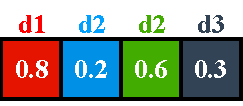
\includegraphics[scale=\scalefigure]{Figures/chap 3/Individual.pdf}
	\caption{A representation of a chromosome}
	\label{fig:individual}
\end{figure}